\documentclass{ximera}

%\usepackage{todonotes}

\newcommand{\todo}{}

\usepackage{tkz-euclide}
\tikzset{>=stealth} %% cool arrow head
\tikzset{shorten <>/.style={ shorten >=#1, shorten <=#1 } } %% allows shorter vectors

\usepackage{tkz-tab}  %% sign charts
\usetikzlibrary{decorations.pathreplacing} 

\usetikzlibrary{backgrounds} %% for boxes around graphs
\usetikzlibrary{shapes,positioning}  %% Clouds and stars
\usetikzlibrary{matrix} %% for matrix
\usepgfplotslibrary{polar} %% for polar plots
\usetkzobj{all}
\usepackage[makeroom]{cancel} %% for strike outs
%\usepackage{mathtools} %% for pretty underbrace % Breaks Ximera
\usepackage{multicol}

\usepackage{polynom}



\usepackage[many]{tcolorbox}  %% for titled boxes
\newtcolorbox{xbox}[1]{%
    tikznode boxed title,
    enhanced,
    arc=0mm,
    interior style={white},
    attach boxed title to top center= {yshift=-\tcboxedtitleheight/2},
    fonttitle=\bfseries,
    colbacktitle=white,coltitle=black,
    boxed title style={size=normal,colframe=white,boxrule=0pt},
    title={#1}}


\usepackage{array}
\setlength{\extrarowheight}{+.1cm}   
\newdimen\digitwidth
\settowidth\digitwidth{9}
\def\divrule#1#2{
\noalign{\moveright#1\digitwidth
\vbox{\hrule width#2\digitwidth}}}





\newcommand{\RR}{\mathbb R}
\newcommand{\R}{\mathbb R}
\newcommand{\N}{\mathbb N}
\newcommand{\Z}{\mathbb Z}

%\renewcommand{\d}{\,d\!}
\renewcommand{\d}{\mathop{}\!d}
\newcommand{\dd}[2][]{\frac{\d #1}{\d #2}}
\newcommand{\pp}[2][]{\frac{\partial #1}{\partial #2}}
\renewcommand{\l}{\ell}
\newcommand{\ddx}{\frac{d}{\d x}}
\newcommand{\ddt}{\frac{d}{\d t}}

\newcommand{\zeroOverZero}{\ensuremath{\boldsymbol{\tfrac{0}{0}}}}
\newcommand{\inftyOverInfty}{\ensuremath{\boldsymbol{\tfrac{\infty}{\infty}}}}
\newcommand{\zeroOverInfty}{\ensuremath{\boldsymbol{\tfrac{0}{\infty}}}}
\newcommand{\zeroTimesInfty}{\ensuremath{\small\boldsymbol{0\cdot \infty}}}
\newcommand{\inftyMinusInfty}{\ensuremath{\small\boldsymbol{\infty - \infty}}}
\newcommand{\oneToInfty}{\ensuremath{\boldsymbol{1^\infty}}}
\newcommand{\zeroToZero}{\ensuremath{\boldsymbol{0^0}}}
\newcommand{\inftyToZero}{\ensuremath{\boldsymbol{\infty^0}}}



\newcommand{\numOverZero}{\ensuremath{\boldsymbol{\tfrac{\#}{0}}}}
\newcommand{\dfn}{\textbf}
%\newcommand{\unit}{\,\mathrm}
\newcommand{\unit}{\mathop{}\!\mathrm}
\newcommand{\eval}[1]{\bigg[ #1 \bigg]}
\newcommand{\seq}[1]{\left( #1 \right)}
\renewcommand{\epsilon}{\varepsilon}
\renewcommand{\iff}{\Leftrightarrow}

\DeclareMathOperator{\arccot}{arccot}
\DeclareMathOperator{\arcsec}{arcsec}
\DeclareMathOperator{\arccsc}{arccsc}
\DeclareMathOperator{\si}{Si}
\DeclareMathOperator{\proj}{proj}
\DeclareMathOperator{\scal}{scal}


\newcommand{\tightoverset}[2]{% for arrow vec
  \mathop{#2}\limits^{\vbox to -.5ex{\kern-0.75ex\hbox{$#1$}\vss}}}
\newcommand{\arrowvec}[1]{\tightoverset{\scriptstyle\rightharpoonup}{#1}}
\renewcommand{\vec}{\mathbf}
\newcommand{\veci}{\vec{i}}
\newcommand{\vecj}{\vec{j}}
\newcommand{\veck}{\vec{k}}
\newcommand{\vecl}{\boldsymbol{\l}}

\newcommand{\dotp}{\bullet}
\newcommand{\cross}{\boldsymbol\times}
\newcommand{\grad}{\boldsymbol\nabla}
\newcommand{\divergence}{\grad\dotp}
\newcommand{\curl}{\grad\cross}
%\DeclareMathOperator{\divergence}{divergence}
%\DeclareMathOperator{\curl}[1]{\grad\cross #1}


\colorlet{textColor}{black} 
\colorlet{background}{white}
\colorlet{penColor}{blue!50!black} % Color of a curve in a plot
\colorlet{penColor2}{red!50!black}% Color of a curve in a plot
\colorlet{penColor3}{red!50!blue} % Color of a curve in a plot
\colorlet{penColor4}{green!50!black} % Color of a curve in a plot
\colorlet{penColor5}{orange!80!black} % Color of a curve in a plot
\colorlet{fill1}{penColor!20} % Color of fill in a plot
\colorlet{fill2}{penColor2!20} % Color of fill in a plot
\colorlet{fillp}{fill1} % Color of positive area
\colorlet{filln}{penColor2!20} % Color of negative area
\colorlet{fill3}{penColor3!20} % Fill
\colorlet{fill4}{penColor4!20} % Fill
\colorlet{fill5}{penColor5!20} % Fill
\colorlet{gridColor}{gray!50} % Color of grid in a plot

\newcommand{\surfaceColor}{violet}
\newcommand{\surfaceColorTwo}{redyellow}
\newcommand{\sliceColor}{greenyellow}




\pgfmathdeclarefunction{gauss}{2}{% gives gaussian
  \pgfmathparse{1/(#2*sqrt(2*pi))*exp(-((x-#1)^2)/(2*#2^2))}%
}


%%%%%%%%%%%%%
%% Vectors
%%%%%%%%%%%%%

%% Simple horiz vectors
\renewcommand{\vector}[1]{\left\langle #1\right\rangle}


%% %% Complex Horiz Vectors with angle brackets
%% \makeatletter
%% \renewcommand{\vector}[2][ , ]{\left\langle%
%%   \def\nextitem{\def\nextitem{#1}}%
%%   \@for \el:=#2\do{\nextitem\el}\right\rangle%
%% }
%% \makeatother

%% %% Vertical Vectors
%% \def\vector#1{\begin{bmatrix}\vecListA#1,,\end{bmatrix}}
%% \def\vecListA#1,{\if,#1,\else #1\cr \expandafter \vecListA \fi}

%%%%%%%%%%%%%
%% End of vectors
%%%%%%%%%%%%%

%\newcommand{\fullwidth}{}
%\newcommand{\normalwidth}{}



%% makes a snazzy t-chart for evaluating functions
%\newenvironment{tchart}{\rowcolors{2}{}{background!90!textColor}\array}{\endarray}

%%This is to help with formatting on future title pages.
\newenvironment{sectionOutcomes}{}{} 



%% Flowchart stuff
%\tikzstyle{startstop} = [rectangle, rounded corners, minimum width=3cm, minimum height=1cm,text centered, draw=black]
%\tikzstyle{question} = [rectangle, minimum width=3cm, minimum height=1cm, text centered, draw=black]
%\tikzstyle{decision} = [trapezium, trapezium left angle=70, trapezium right angle=110, minimum width=3cm, minimum height=1cm, text centered, draw=black]
%\tikzstyle{question} = [rectangle, rounded corners, minimum width=3cm, minimum height=1cm,text centered, draw=black]
%\tikzstyle{process} = [rectangle, minimum width=3cm, minimum height=1cm, text centered, draw=black]
%\tikzstyle{decision} = [trapezium, trapezium left angle=70, trapezium right angle=110, minimum width=3cm, minimum height=1cm, text centered, draw=black]


\outcome{Use integral notation for both antiderivatives and definite integrals.}
\outcome{Compute definite integrals using geometry.}
\outcome{Compute definite integrals using the properties of integrals.}
\outcome{Justify the properties of definite integrals using algebra or geometry.}
\outcome{Understand how Riemann sums are used to find exact area.}
\outcome{Define net area.}
\outcome{Split the area under a curve into several pieces to aid with calculations.}
\outcome{Use symmetry to calculate definite integrals.}
\outcome{Explain geometrically why symmetry of a function simplifies calculation of some definite integrals.}


\title[Dig-In:]{The definite integral}

\begin{document}
\begin{abstract}
  Definite integrals compute signed area.
\end{abstract}
\maketitle


In the previous sections, we've been approximating the area under a curve by treating the region as a collection of
rectangles. 

\begin{example}
	Approximate the area under the graph of $f(x)=x^2$ on the interval $[0,1]$ using right-endpoints and $n$ rectangles, for $n$ a positive integer.
	\begin{explanation}
		We'll start with the widths: $\Delta x = \frac{b-a}{n} = \frac{1}{n}$.
		
		Since we're using right-endpoints, the sample points are given by $x_k^* = a + k \Delta x = \frac{k}{n}$.
		
		The height of the $k$-th rectangle is $f(x_k^*) = \left( \frac{k}{n} \right)^2 = \frac{\answer[given]{k^2}}{n^2}$.
		
		The area of the $k$-th rectangle is $f(x_k^*)\Delta x = \left(\frac{k^2}{n^2}\right)\left( \frac{1}{n} \right) = \frac{\answer[given]{k^2}}{\answer[given]{n^3}}$.
		
		The area approximation is given by the Riemann sum.
		\begin{align*}
			\sum_{k=1}^{n} f(x_k^*) \Delta x &= \sum_{k=1}^n \frac{k^2}{n^3}\\
				&= \frac{1}{n^3} \sum_{k=1}^{n} \answer[given]{k^2} \quad \text{(We have a formula for this!)}\\
				&= \frac{1}{n^3} \left( \frac{n(n+1)(2n+1)}{6}\right)\\
				&= \frac{n(n+1)(2n+1)}{6n^3}\\
				&= \frac{(n+1)(2n+1)}{6n^2}
		\end{align*}

		The approximate area is $\frac{(n+1)(2n+1)}{6n^2}$.
	\end{explanation}
\end{example}

The benefit of doing this calculation with $n$ still variable, is that it's now easy to find the approximation for every possible value of $n$!
If we wanted to approximate the area under $f(x)=x^2$ using $4$ rectangles, we could substitute $n=4$ into this formula.
$\frac{(4+1)(2\cdot4+1)}{6(4)^2} = \frac{15}{32}$.  If we wanted to use $10$ rectangles, we can substitute $n=10$ into it.
$\frac{(10+1)(2\cdot 10+1)}{6(10)^2} = \frac{77}{200}$.

Why would we want to be able to plug in different values of $n$?  Remember how we made the approximation better and better?  By taking
more and more rectangles!  The actual area is given in the limit as $n\to \infty$.

\begin{example}
	Find the actual area under the graph of $f(x)=x^2$ on the interval $[0,1]$.
	\begin{explanation}
		We saw that the area approximation using $n$ rectangles was given by
		\[ A(n) = \frac{(n+1)(2n+1)}{6n^2} \]
		The actual area is given by
		\begin{align*}
			\lim_{n\to\infty} A(n) &= \lim_{n\to\infty} \frac{(n+1)(2n+1)}{6n^2}\\
				&= \lim_{n\to\infty} \frac{2n^2+3n+1}{6n^2} \\
				&= \lim_{n\to\infty} \frac{4n+3}{12n} \quad \text{L'H\^opital's Rule}\\
				&= \lim_{n\to\infty} \frac{4}{12} \quad \text{L'H\^opital's Rule}\\
				&= \answer{\frac{1}{3}}
		\end{align*}
	\end{explanation}
\end{example}

All of the functions we have been examining have been positive.  What changes if $f$ is negative in the region?



Definite integrals, often simply called integrals, compute signed area. 

\begin{definition}\index{integral}\index{definite integral}
The \dfn{definite integral}
\[
\int_a^b f(x) \d x
\]
computes the signed area between $y=f(x)$ and the $x$-axis on the
interval $[a,b]$.
\begin{itemize}
  \item If the region is above the $x$-axis, then the area has
    positive sign.
  \item If the region is below the $x$-axis, then the area has
    negative sign.
\end{itemize}
Note, when working with signed area, ``positive'' and ``negative''
area cancel each other out.
\end{definition}

\begin{question}
Consider the following graph of $y=f(x)$:
\begin{image}
  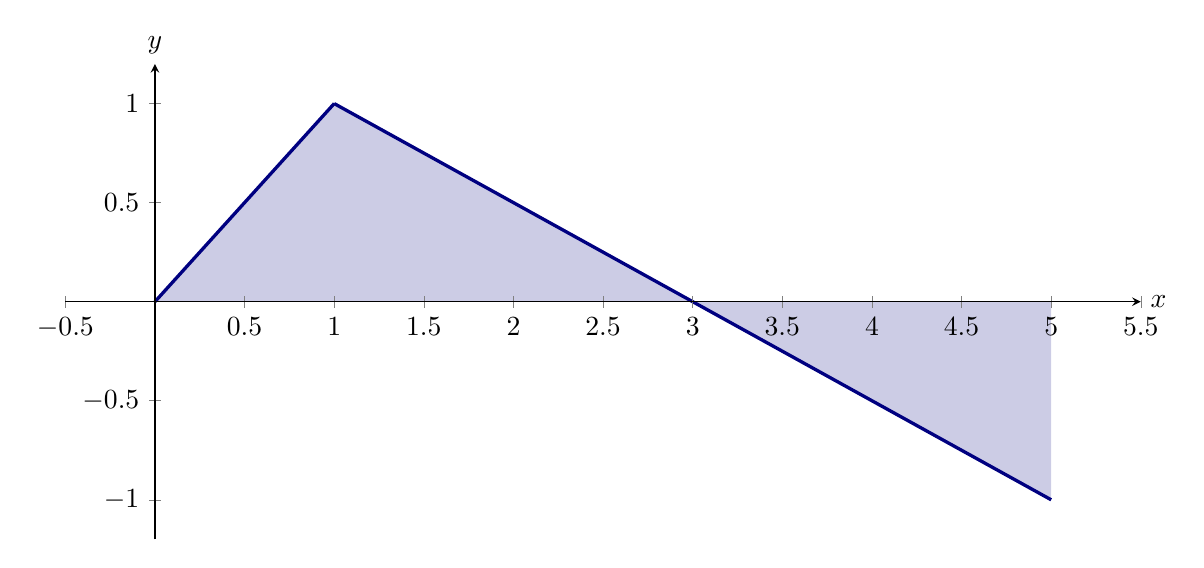
\begin{tikzpicture}
    \begin{axis}[
        width=6in,
        height=3in,
        xmin=-.5, xmax=5.5,ymin=-1.2,ymax=1.2,domain=0:6,
        axis lines =center, xlabel=$x$, ylabel=$y$,
        every axis y label/.style={at=(current axis.above origin),anchor=south},
        every axis x label/.style={at=(current axis.right of origin),anchor=west},
        axis on top,
    ] 
      \addplot [draw=none, %pattern=north west lines, pattern color=blue,
        fill=fillp,
        domain=0:1] {x} \closedcycle;
      \addplot [draw=none, %pattern=north west lines, pattern color=blue,
        fill=fillp,
        domain=1:5] {1.5-x/2} \closedcycle;
      
      \addplot [penColor,very thick,domain=0:1] {x};
      \addplot [penColor,very thick,domain=1:5] {1.5-x/2};
  \end{axis}
  \end{tikzpicture}
\end{image}
Compute:
\begin{enumerate}
\item $\int_0^3 f(x) \d x \begin{prompt}= \answer{1.5}\end{prompt}$
\item $\int_3^5 f(x) \d x \begin{prompt}= \answer{-1}\end{prompt}$
\item $\int_0^5 f(x) \d x \begin{prompt}= \answer{0.5}\end{prompt}$
\item $\int_0^3 5\cdot f(x) \d x \begin{prompt}= \answer{7.5}\end{prompt}$
\item $\int_1^1 5\cdot f(x) \d x \begin{prompt}= \answer{0}\end{prompt}$
\end{enumerate}
\begin{hint}
  Use the formula for the area of a triangle.
\end{hint}
\begin{hint}
  Remember, we are dealing with ``signed'' area here:
  \begin{image}
  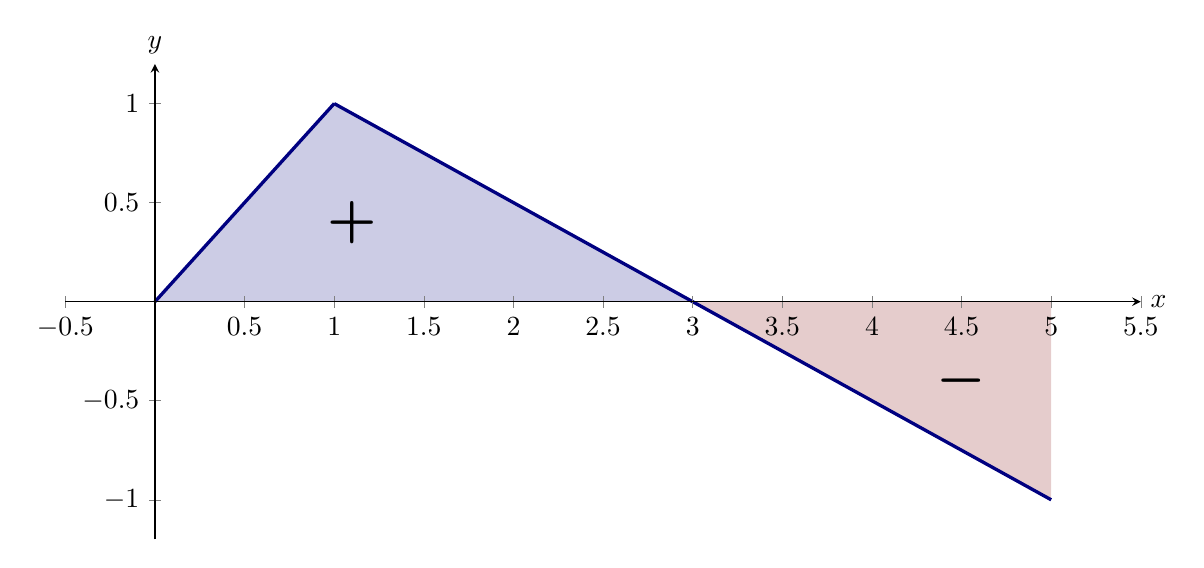
\begin{tikzpicture}
    \begin{axis}[
        width=6in,
        height=3in,
        xmin=-.5, xmax=5.5,ymin=-1.2,ymax=1.2,domain=0:6,
        axis lines =center, xlabel=$x$, ylabel=$y$,
        every axis y label/.style={at=(current axis.above origin),anchor=south},
        every axis x label/.style={at=(current axis.right of origin),anchor=west},
        axis on top,
    ] 
      \addplot [draw=none, fill=fillp,domain=0:1] {x} \closedcycle;
      \addplot [draw=none, fill=fillp,domain=1:3] {1.5-x/2} \closedcycle;
      \addplot [draw=none, fill=filln,domain=3:5] {1.5-x/2} \closedcycle;
      
      \addplot [penColor,very thick,domain=0:1] {x};
      \addplot [penColor,very thick,domain=1:5] {1.5-x/2};
      \node at (axis cs:1.1,.4) [textColor] {\scalebox{2}{$\boldsymbol+$}};
      \node at (axis cs:4.5,-.4) [textColor] {\scalebox{2}{$\boldsymbol-$}};
  \end{axis}
  \end{tikzpicture}
\end{image}
\end{hint}
\end{question}


Our previous question hopefully gives us enough insight that this next
theorem is unsurprising.

\begin{theorem}[Properties of the definite integral]
Let $f$ and $g$ be defined on a closed interval $[a,b]$ that contains the
value $c$, and let $k$ be a constant. The following
hold:
\begin{enumerate}
\item $\int_a^a f(x)\d x = 0$
\item $\int_a^c f(x)\d x + \int_c^b f(x)\d x = \int_a^b f(x)\d x$
\item $\int_a^bf(x)\d x = -\int_b^a f(x)\d x$
\item $\int_a^b f(x)\pm g(x)\d x = \int_a^bf(x)\d x \pm \int_a^bg(x)\d x$
\item $\int_a^bk\cdot f(x)\d x = k\cdot\int_a^bf(x)\d x$
\end{enumerate}
\begin{explanation}
  We will address each property in turn:
\begin{enumerate}
\item Here, there is no ``area under the curve'' when the region has
  no width; hence this definite integral is $0$.
\item This states that total area is the sum of the areas of
  subregions. Here a picture is worth a thousand words:
  \begin{image}
    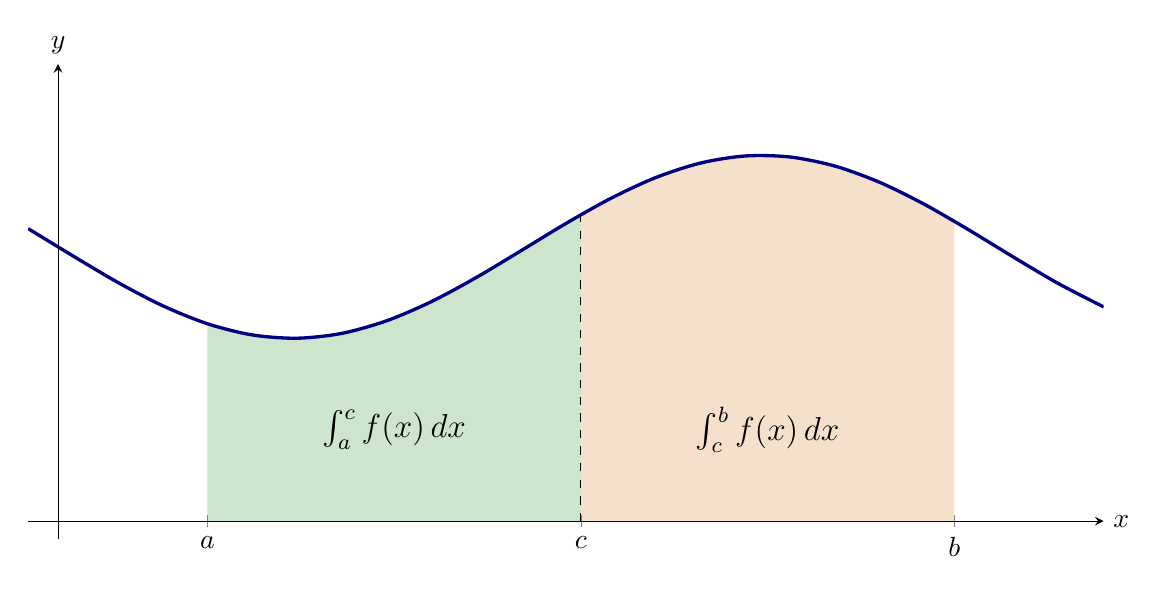
\begin{tikzpicture}[
        declare function = {f(\x) = -sin(deg(\x)) + 3;} ]
      \begin{axis}[
          domain=-.2:7, xmin =-.2,xmax=7,ymax=5,ymin=-.2,
          width=6in,
          height=3in,
          xtick={1,3.5,6}, 
          xticklabels={$a$,$c$,$b$},
          ytick style={draw=none},
          yticklabels={},
          axis lines=center, xlabel=$x$, ylabel=$y$,
          every axis y label/.style={at=(current axis.above origin),anchor=south},
          every axis x label/.style={at=(current axis.right of origin),anchor=west},
          axis on top,
          ]
        \addplot [draw=none,fill=fill4,domain=1:3.5, smooth] {f(x)} \closedcycle;
        
        \addplot [draw=none,fill=fill5,domain=3.5:6, smooth] {f(x)} \closedcycle;
        
        \addplot [very thick,penColor, smooth] {f(x)};
        \addplot [dashed] plot coordinates {(3.5,0) (3.5,{f(3.5)})};
        
        \node at (axis cs:2.25,1) {\large$\int_a^c f(x)\d x$};
        \node at (axis cs:4.75,1) {\large$\int_c^b f(x)\d x$};
      \end{axis}
    \end{tikzpicture}
  \end{image}		
  It is important to note that this still holds true even if
  $a<b<c$. We discuss this in the next point.
  
\item For now, this property can be viewed a merely a convention to
  make other properties work well. However, later we will see how this
  property has a justification all its own.

\item This states that when one scales a function by, for instance, $7$,
  the area of the enclosed region also is scaled by a factor of
  $7$.
\item This states that the integral of the sum is the sum of the
  integrals.
\end{enumerate}
\end{explanation}
\end{theorem}

Due to the geometric nature of integration, geometric properties of
functions can help us compute integrals.

\begin{example}
  Compute:
  \[
  \int_0^6 |x-3| \d x
  \]
  \begin{explanation}
    This may seem difficult at first. Perhaps the first thing to do is
    look at a graph of $y=x-3$:
  \begin{image}
  \begin{tikzpicture}
    \begin{axis}[
        width=6in,
        height=3in,
        xmin=-.5, xmax=6.5,ymin=-4,ymax=4,domain=0:6,
        axis lines =center, xlabel=$x$, ylabel=$y$,
        every axis y label/.style={at=(current axis.above origin),anchor=south},
        every axis x label/.style={at=(current axis.right of origin),anchor=west},
        axis on top,
    ] 
      \addplot [penColor,very thick,domain=0:6] {x-3};
    \end{axis}
  \end{tikzpicture}
    \end{image}
    Now we can graph $y=|x-3|$:
    \begin{image}
  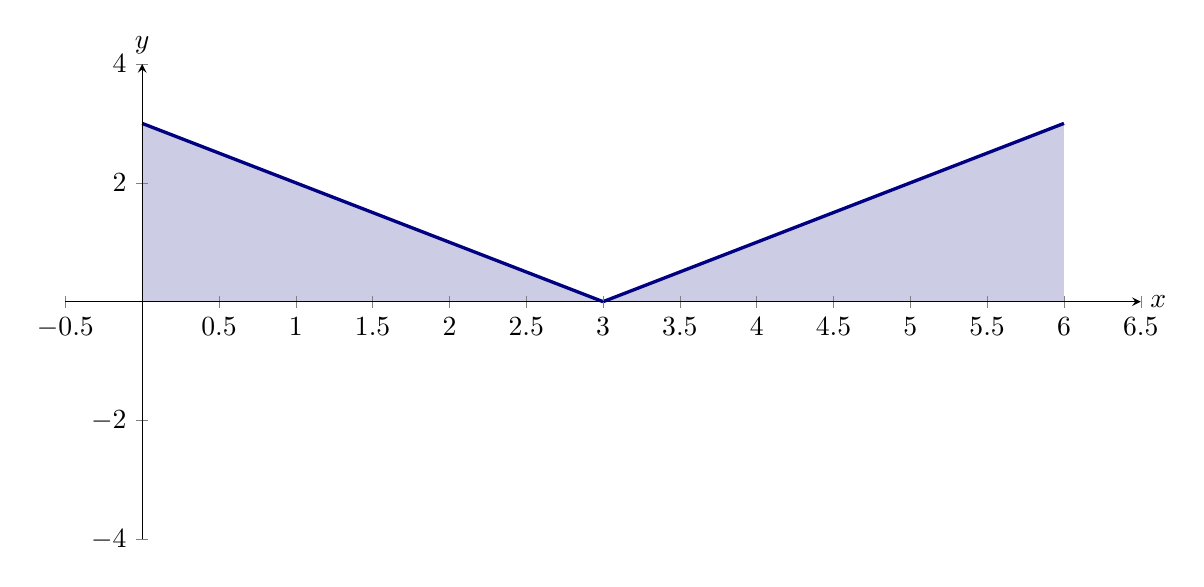
\begin{tikzpicture}
    \begin{axis}[
        width=6in,
        height=3in,
        xmin=-.5, xmax=6.5,ymin=-4,ymax=4,domain=0:6,
        axis lines =center, xlabel=$x$, ylabel=$y$,
        every axis y label/.style={at=(current axis.above origin),anchor=south},
        every axis x label/.style={at=(current axis.right of origin),anchor=west},
        axis on top,
    ] 
      \addplot [draw=none, fill=fillp,domain=0:3] {3-x} \closedcycle;
      \addplot [draw=none, fill=fillp,domain=3:6] {x-3} \closedcycle;
      \addplot [penColor,very thick,domain=3:6] {x-3};
      \addplot [penColor,very thick,domain=0:3] {3-x};
    \end{axis}
  \end{tikzpicture}
    \end{image}
    Now we see that we really have two triangles, each with base $3$
    and height $3$.  Hence
    \begin{align*}
    \int_0^6 |x-3| \d x &= \int_0^3 \answer[given]{3-x} \d x + \int_3^6 \answer[given]{x-3} \d x\\
    &= \frac{3\cdot 3}{2} + \frac{3\cdot 3}{2}\\
    &=\answer[given]{9}.
    \end{align*}
  \end{explanation}
\end{example}

\begin{definition}
  A function $f$ is an \dfn{odd} function if
  \[
  f(-x) = -f(x),
  \]
  and a function $g$ is an \dfn{even} function if
  \[
  g(-x) = g(x).
  \]
\end{definition}

The names \textit{odd} and \textit{even} come from the fact that these
properties are shared by functions of the form $x^n$ where $n$ is
either odd or even. For example, if $f(x) = x^3$, then
\[
f(-7) = -f(7),
\]
and if $g(x) = x^4$, then
\[
g(-7) = g(7).
\]
Geometrically, even functions have \textit{horizontal
  symmetry}. Cosine is an even function:
\begin{image}
 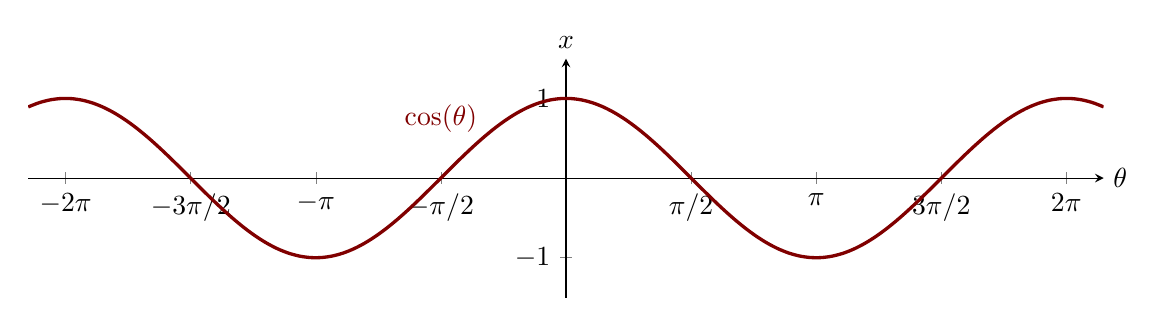
\begin{tikzpicture}
	\begin{axis}[
            xmin=-6.75,xmax=6.75,ymin=-1.5,ymax=1.5,
            axis lines=center,
            xtick={-6.28, -4.71, -3.14, -1.57, 0, 1.57, 3.142, 4.71, 6.28},
            xticklabels={$-2\pi$,$-3\pi/2$,$-\pi$, $-\pi/2$, $0$, $\pi/2$, $\pi$, $3\pi/2$, $2\pi$},
            ytick={-1,1},
            %ticks=none,
            width=6in,
            height=3in,
            unit vector ratio*=1 1 1,
            xlabel=$\theta$, ylabel=$x$,
            every axis y label/.style={at=(current axis.above origin),anchor=south},
            every axis x label/.style={at=(current axis.right of origin),anchor=west},
          ]        
          \addplot [very thick, penColor2, samples=100,smooth, domain=(-6.75:6.75)] {cos(deg(x))};
          \node at (axis cs:-1.57,.75) [penColor2] {$\cos(\theta)$};
        \end{axis}
\end{tikzpicture}
\end{image}
On the other hand, odd functions have $180^\circ$ \textit{rotational symmetry}
around the origin. Sine is an odd function:
\begin{image}
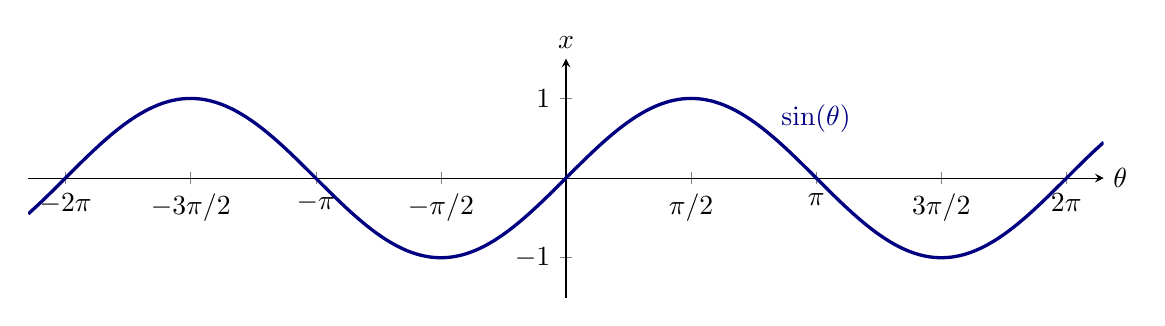
\begin{tikzpicture}
	\begin{axis}[
            xmin=-6.75,xmax=6.75,ymin=-1.5,ymax=1.5,
            axis lines=center,
            xtick={-6.28, -4.71, -3.14, -1.57, 0, 1.57, 3.142, 4.71, 6.28},
            xticklabels={$-2\pi$,$-3\pi/2$,$-\pi$, $-\pi/2$, $0$, $\pi/2$, $\pi$, $3\pi/2$, $2\pi$},
            ytick={-1,1},
            %ticks=none,
            width=6in,
            height=3in,
            unit vector ratio*=1 1 1,
            xlabel=$\theta$, ylabel=$x$,
            every axis y label/.style={at=(current axis.above origin),anchor=south},
            every axis x label/.style={at=(current axis.right of origin),anchor=west},
          ]        
          \addplot [very thick, penColor, samples=100,smooth, domain=(-6.75:6.75)] {sin(deg(x))};
          
          \node at (axis cs:3.14,.75) [penColor] {$\sin(\theta)$};
        \end{axis}
\end{tikzpicture}
\end{image}
\begin{question}
  Let $f$ be an odd function defined for all real numbers. Compute:
  \[
  \int_{-2}^2 f(x) \d x \begin{prompt}=\answer{0}\end{prompt}
  \]
  \begin{hint}
    Since our function is odd, it must look something like:
    \begin{image}
      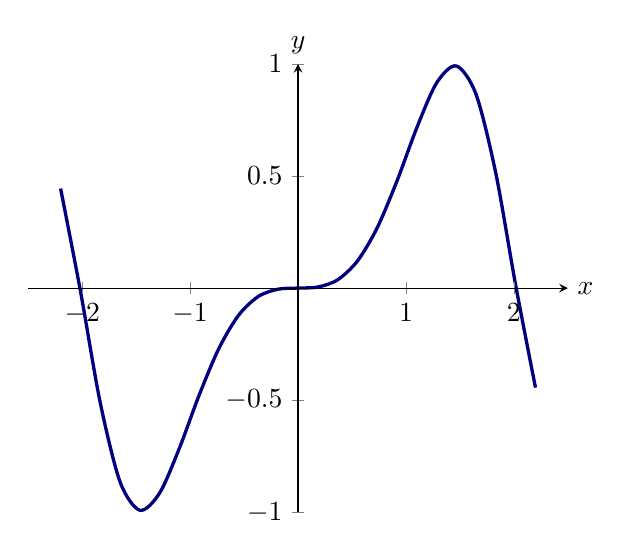
\begin{tikzpicture}
        \begin{axis}[
            xmin=-2.5, xmax=2.5,ymin=-1,ymax=1,domain=-2.2:2.2,
            axis lines =center, xlabel=$x$, ylabel=$y$,
            every axis y label/.style={at=(current axis.above origin),anchor=south},
            every axis x label/.style={at=(current axis.right of origin),anchor=west},
            axis on top,
          ] 
          \addplot [penColor,very thick,smooth] {sin(deg(x))*sin(deg(x^2/1.3))};
        \end{axis}
      \end{tikzpicture}
    \end{image}
  \end{hint}
  \begin{hint}
    The integral above computes the following (signed) area:
    \begin{image}
      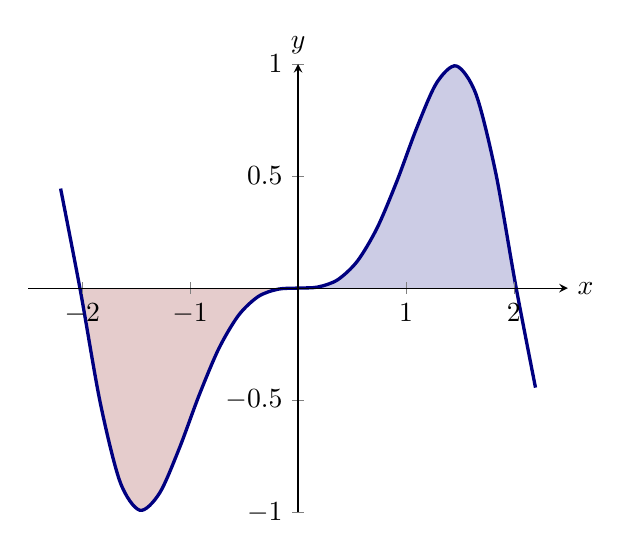
\begin{tikzpicture}
        \begin{axis}[
            xmin=-2.5, xmax=2.5,ymin=-1,ymax=1,domain=-2.2:2.2,
            axis lines =center, xlabel=$x$, ylabel=$y$,
            every axis y label/.style={at=(current axis.above origin),anchor=south},
            every axis x label/.style={at=(current axis.right of origin),anchor=west},
            axis on top,
          ]
          \addplot [draw=none,fill=fillp,domain=0:2, smooth] {sin(deg(x))*sin(deg(x^2/1.3))} \closedcycle;
          \addplot [draw=none,fill=filln,domain=-2:0, smooth] {sin(deg(x))*sin(deg(x^2/1.3))} \closedcycle;
          \addplot [penColor,very thick,smooth] {sin(deg(x))*sin(deg(x^2/1.3))};
        \end{axis}
      \end{tikzpicture}
    \end{image}
  \end{hint}
\end{question}


\begin{question}
  Let $f$ be an odd function defined for all real numbers. Which of
  the following are equal to
  \[
  \int_2^4 f(x) \d x ?
  \]
  \begin{selectAll}
    \choice{$\int_{4}^{2} f(x) \d x$}
    \choice{$\int_{-4}^{-2} f(x) \d x$}
    \choice[correct]{$\int_{-2}^{-4} f(x) \d x$}
    \choice[correct]{$\int_{-2}^{4} f(x) \d x$}
    \choice{$\int_{4}^{-2} f(x) \d x$}
    \choice[correct]{$\int_{2}^{-4} f(x) \d x$}
    \choice{$\int_{-4}^{2} f(x) \d x$}
    \choice[correct]{$-\int_{-4}^{2} f(x) \d x$}
    \choice[correct]{$-\int_{-4}^{-2} f(x) \d x$}
  \end{selectAll}
\end{question}




\section{Signed verses geometric area}


We know that the signed area between a curve $y=f(x)$ and the $x$-axis
on $[a,b]$ is given by
\[
\int_a^b f(x) \d x.
\]
On the other hand, if we want to know the \textit{geometric area},
meaning the ``actual'' area, we compute
\[
\int_a^b |f(x)| \d x.
\]
\begin{question}
  True or false:
  \[
  \int_a^b |f(x)| \d x = \left|\int_a^b f(x) \d x\right|
  \]
  \begin{multipleChoice}
    \choice{true}
    \choice[correct]{false}
  \end{multipleChoice}
  \begin{feedback}
    Consider $f(x) = x^3$ on the interval $[-1,1]$. Here
    \[
    \int_a^b |f(x)| \d x = 1/2 \qquad\text{but}\qquad \left|\int_a^b
    f(x) \d x\right| = 0.
    \]
  \end{feedback}
\end{question}



\section{Integrals and Riemann sums}

Exactly how does an integral compute area? It depends on who you
ask. If you ask Riemann, then you set
\[
\Delta x = \frac{b-a}{n}
\]
and look at the following limit of Riemann sums:
\[
\lim_{n\to \infty} \sum_{k=1}^n f(x_k^*) \Delta x = \int_a^b f(x) \d x.
\]
This says, take a curve, slice it up into $n$ pieces on the interval
$[a,b]$, add up all the areas of rectangles whose width is determined
by the slices and the height is determined by a sample point in one of
these pieces.

\begin{example}
  Compute this limit:
  \[
  \lim_{n\to \infty} \sum_{k=1}^n \left(\sqrt{1-\left(-1+\frac{2k}{n}\right)^2}\right)
  \left(\frac{2}{n}\right)
  \]
  \begin{explanation}
    This is a limit of Riemann sums!  Specifically, it is a limit of
    Riemann sums of $n$ rectangles, where
    \[
    \Delta x = \answer[given]{\frac{2}{n}}
    \]
    and
    \[
    x_k^* = -1+\frac{2k}{n}.
    \]
    Hence, we may rewrite this as
    \[
    \lim_{n\to \infty} \sum_{k=1}^n \left(\sqrt{1-(x_k^*)^2}\right)
    \Delta x.
    \]
    Now we see that this computes the area between the $x$-axis and
    the curve $y = \sqrt{1-x^2}$. Let's see it:
    \begin{image}
  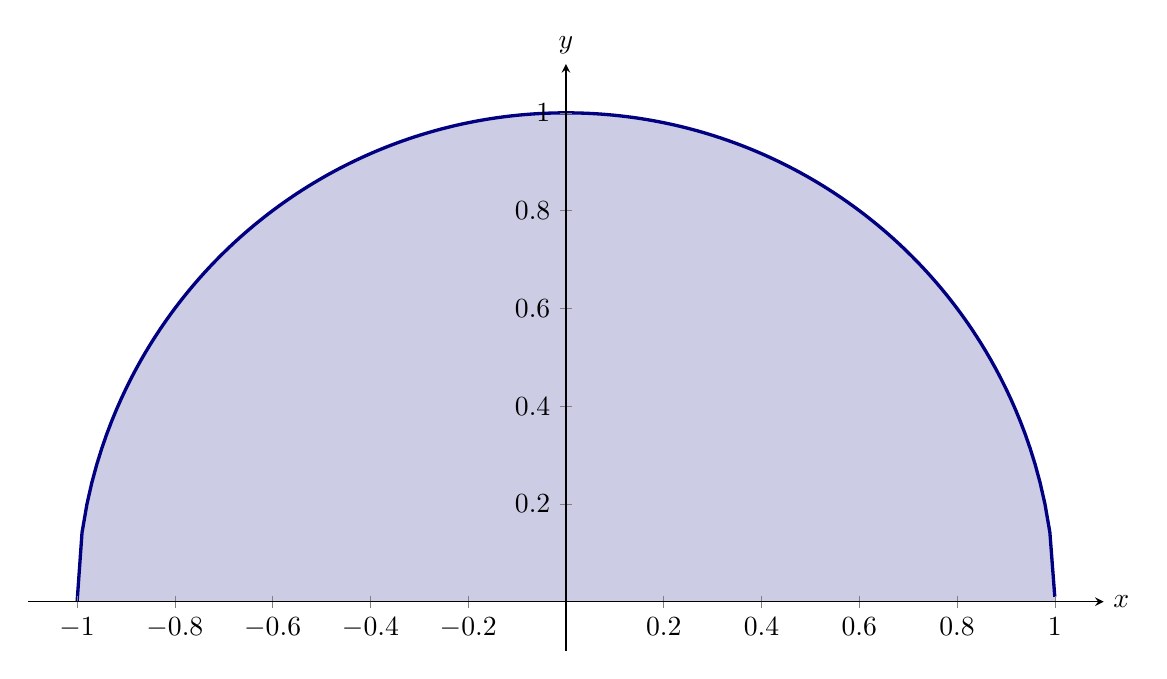
\begin{tikzpicture}
    \begin{axis}[
        width=6in,
        %height=3in,
        unit vector ratio*=1 1 1,            
        xmin=-1.1, xmax=1.1,ymin=-.1,ymax=1.1,
        axis lines =center, xlabel=$x$, ylabel=$y$,
        every axis y label/.style={at=(current axis.above origin),anchor=south},
        every axis x label/.style={at=(current axis.right of origin),anchor=west},
        axis on top,
    ] 
      \addplot [draw=none, fill=fillp,samples=200,domain=-1:1] {sqrt(1-x^2)} \closedcycle;
      
      \addplot [penColor,very thick,samples=200,domain=-1:1] {sqrt(1-x^2)};
    \end{axis}
  \end{tikzpicture}
    \end{image}
    By geometry, we know that this semicircle has area $\answer[given]{\pi/2}$. Hence
    \[
    \lim_{n\to \infty} \sum_{k=1}^n \left(\sqrt{1-(x_k^*)^2}\right)\Delta x =\answer[given]{\pi/2}.
    \]
  \end{explanation}
\end{example}



\end{document}
